\documentclass[11pt,letter]{article}
\usepackage[top=1.00in, bottom=1.0in, left=1.1in, right=1.1in]{geometry}
\renewcommand{\baselinestretch}{1.6}
\usepackage{graphicx}
\usepackage{natbib}
\usepackage{amsmath}
\usepackage{amssymb} 
\usepackage{lineno}
\usepackage{xr-hyper}
\externaldocument{decsens_supp}
% \externaldocument{letters/plosbio_r1/decsens_plosbio1_p2}
\newcommand{\R}[1]{\label{#1}\linelabel{#1}}
\usepackage{hyperref}

\def\labelitemi{--}
\parindent=0pt
\begin{document}

\title{A simple explanation for declining temperature sensitivity \\ with warming} % The illusion of declining temperature sensitivity with warming // Sensitivities are not declining with warming OR As climate change accelerates biology, chasing statistical artifacts ensues
\author{E. M. Wolkovich$^{1,a}$,  J. L. Auerbach$^{2}$, C. J. Chamberlain$^{3}$, D. M. Buonaiuto$^{3}$, \\ A. K. Ettinger$^4$, I. Morales-Castilla$^{5}$ \& A. Gelman$^{2}$} 
\date{} %\today
\maketitle
$^1$Forest \& Conservation Sciences, Faculty of Forestry, University of British Columbia, Vancouver, British Columbia, Canada\\
$^2$Department of Statistics, Columbia University, New York, NY 10027, USA\\
$^3$Department of Organismic and Evolutionary Biology, Harvard University, Cambridge, Massachusetts, USA\\
$^4$The Nature Conservancy in Washington, 74 Wall Street, Seattle, WA, USA\\
$^5$GloCEE -- Global Change Ecology and Evolution Group, Department of Life Sciences, University of Alcal\`a CTRA N-II, KM., 33,600, 28802, Alcal\`a de Henares, Spain\\
$^a$Corresponding author (ORCID: 0000-0001-7653-893X); e.wolkovich@ubc.ca; 604.827.5246
\vspace{3ex}

\emph{Running title:} Declining temperature sensitivity\\
\emph{Article type}: Perspective\\
% \emph{One sentence summary:} Declining temperature sensitivity with warming is the expected outcome of current methods, not evidence of changing biology.
% Observations of global declines in temperature sensitivity of biological events with climate change have been used as evidence of fundamental shifts in underlying biological processes, but may more simply be explained by the statistical methods used to calculate temperature sensitivity. 

% Phones: Auerbach (dept): 212.851.2132, Holbrook Lab: 617.496-3580, Ailene: 781-296-4821, Nacho: 34 672 74 8160, Gelman: 212-851-2142
% Emails:  jla2167@columbia.edu, cchamberlain@g.harvard.edu, dbuonaiuto@g.harvard.edu, ailene.ettinger@tnc.org, ignacio.moralesc@uah.es, gelman@stat.columbia.edu

% Abstract for longer-form journals ...
% Temperature sensitivity---the magnitude of a biological response per $^{\circ}$C---is a fundamental concept across scientific disciplines, especially biology, where temperature determines the rate of many plant, animal and ecosystem processes. Recently, multiple studies have found temperature sensitivities decline as temperatures rise. Such observations have been used to suggest climate change is reshaping biological processes, with major implications for forecasts of future change. Here we present a simple alternative explanation for observed declining sensitivities: the use of linear models to estimate non-linear temperature responses. We show how linear estimates of sensitivities will appear to decline with warming for events that occur after a cumulative thermal threshold is met---a common model for many biological events. Corrections for the non-linearity of temperature response in simulated data and long-term phenological data from Europe remove the apparent decline. Our results show that rising temperatures combined with linear estimates based on calendar time produce observations of declining sensitivity---without any shift in the underlying biology. Current methods may thus undermine efforts to identify when and how warming will reshape biological processes.
% \emph{Significance statement}: Recently a growing body of literature has observed declining temperature sensitivities of plant leafout and other events with higher temperatures. Such results suggest that climate change is already reshaping fundamental biological processes. These temperature sensitivities are often estimated as the magnitude of a biological response per $^{\circ}$C from linear regression. The underlying model for many events---that a critical threshold of warmth must be reached to trigger the event---however, is non-linear. We show that this mismatch between the statistical and biological models can produce the illusion of declining sensitivities with warming using current methods. We suggest simple alternative approaches that can better identify when and how warming will reshape biological processes.
% 100 word abstract
% Recently a growing body of literature has reported declining phenological sensitivities ($\Delta$ days per $^{\circ}$C) with higher temperatures. Such results suggest that climate change is already reshaping fundamental biological processes. Here we show that these results may simply be the outcome of using linear models to estimate non-linear temperature responses, specifically for events that occur after a cumulative thermal threshold is met---a common model for many biological events. Corrections for the non-linearity of temperature responses consistently remove the apparent decline. Our results suggest that current methods may undermine efforts to identify when and how warming will reshape biological processes.

\newpage
\begin{abstract} % 132 words
Recently, multiple studies have reported declining phenological sensitivities ($\Delta$ days per $^{\circ}$C) with higher temperatures. Such observations have been used to suggest climate change is reshaping biological processes, with major implications for forecasts of future change. Here we show that these results may simply be the outcome of using linear models to estimate non-linear temperature responses, specifically for events that occur after a cumulative thermal threshold is met---a common model for many biological events. Corrections for the non-linearity of temperature responses consistently remove the apparent decline. Our results show that rising temperatures combined with linear estimates based on calendar time produce observations of declining sensitivity---without any shift in the underlying biology. Current methods may thus undermine efforts to identify when and how warming will reshape biological processes.
\end{abstract}
% Recently, a growing body of literature in global change biology has found temperature sensitivities decline as temperatures rise \citep{fu2015,gusewell2017,piao2017,dai2019ag}. These declines are generally attributed to shifts in underlying biological processes caused by warming, yet to date there is no clear evidence of mechanistic changes.
% https://english.stackexchange.com/questions/357736/can-negative-numbers-be-called-large

% Explain the significance of the research at a level understandable to an undergraduate-educated scientist outside their field of specialty; Include no more than 120 words (113 now)
\vspace{5ex}


\newpage
% \linenumbers
\section{Main text} % 1103 right now; ack: 66; datacode: 44; author contr: 41
Climate change has reshaped biological processes around the globe, with shifts in the timing of major life history events (phenology), carbon dynamics and other ecosystem processes. With rising temperatures,  a growing body of literature has documented changes in temperature sensitivity---the magnitude of a biological response scaled per $^{\circ}$C. Many studies have found declining responses to temperature in recent decades \citep{fu2015,piao2017} or lower sensitivities in warmer, urban areas \citep{meng2020}.\\

Most studies attribute changes in temperature sensitivity to shifts in underlying biological processes. Researchers have suggested weaker temperature sensitivities are evidence of increased light limitation in the tundra \citep{piao2017}, or a decline in the relative importance of warm spring temperatures for spring phenological events (e.g., leafout, insect emergence) in the temperate zone \citep{fu2015,meng2020}, as other environmental triggers (e.g., winter temperatures that determine `chilling') play a larger role. Yet, despite an increase in studies reporting declining or shifting temperature sensitivities, none have provided strong evidence of the biological mechanisms underlying these changes  \citep[e.g.,][]{fu2015,meng2020}. The missing mechanisms may be hidden in the data: environmental factors moderate biological processes in complex ways \citep{chuine2016}, are strongly correlated in nature \citep[e.g.,][]{fu2015}, and temperature variance shifts over time and space \citep{keenan2019}. \\
%  fundamental science suggests that warm spring temperatures are the main controller of many temperate phenological events (e.g., leafout, insect emergence), but winter temperatures and photoperiod can also determine the timing of events. Thus, an increased role of winter temperatures or photoperiod could explain observed declines in the temperature sensitivity of plant phenology with warming. 
% ... fundamental science predicts declines in the temperature sensitivity of temperate plant phenology, as the role of spring temperature diminishes relative to the increasing importance of winter temperatures and daylength... For example, the temperature sensitivity of spring leafout may decline if warmer winters mean plants fail to receive enough winter chilling.  

Here we propose a simpler alternative explanation: the use of linear models for non-linear responses to temperature. Researchers generally use methods with assumptions of linearity to calculate temperature sensitivities, often relying on some form of linear regression to compute a change in a quantity---days to leafout or carbon sequestered over a fixed time, for example---per $^{\circ}$C, thus ignoring that many biological responses to temperature, especially events, are non-linear (Fig. \ref{fig:ospreewsims}). \\ % We show, theoretically then with simulated and empirical data, how the use of linear methods for non-linear responses can produce an illusion that the mechanisms underlying biological processes are changing.\\ % We demonstrate this theoretically using first-hitting-time models---and empirically---using both simulated data and long-term phenological data from Europe.\\

Many observed biological responses are the result of continuous non-linear processes that depend on temperature, which are discretized into temporal units for measurement. For example, a biological response, such as leafout, occurs when a certain thermal sum is reached, and plants will reach this threshold more quickly---in calendar time---when average daily temperatures are warmer \citep[Fig. \ref{fig:ospreewsims},][]{kramer2012book}. 
Biologically, however, the plants require the same temperature sum to trigger leafout at high and low average temperatures. Indeed any process observed or measured as the time until reaching a threshold is inversely proportional to the speed at which that threshold is approached. \\ % Climate change steps on the accelerator of biological time, while researchers continue to use calendar time. 

Temperature determines the speed of many biological processes. Thus, at very low temperatures plants would never leaf out and at higher temperatures they could leaf out in only a matter of days---yet sensitivities estimated from linear regression at higher (warmer) temperatures would appear much lower than those observed at lower temperatures. Using a simple model where leafout occurs after a thermal sum is met we can hold the temperature threshold for leafout constant \citep{zohner2020gcb} and examine how estimated sensitivities (measured in days per $^{\circ}$C using linear regression) shift with warming. In this simple thermal sum model \citep[which we argue is the null model for studies of biological events across different temperatures, Fig. \ref{fig:ospreewsims} and][]{kramer2012book,zohner2020gcb} we find declining sensitivities with warming (Fig \ref{fig:basicsims}; see `A first-hitting-time model of leafout' in Supporting Information for a full derivation of the statistical properties). Indeed, under this model constant temperature sensitivity would be evidence that the temperature threshold is not constant and the mechanisms underlying the leafout process have changed. \\
% show this by deriving the relationship between a biological response and temperature using a simple stochastic model, which describes the first time a random process hits a threshold Our model holds the temperature threshold for leafout constant \citep{Hunter:1992jw,zohner2020gcb}. Even though the mechanism by which temperature leads to leafout does not change, the model produces declining sensitivity---as measured in days per $^{\circ}$C---with warming. Indeed, under this model constant temperature sensitivity would be evidence that the temperature threshold is not constant and the mechanisms underlying the leafout process have changed. \\ % We consider two common scenarios: one measuring average daily temperature up until the leafout date, and the other measuring average daily temperature over a fixed window (such as March 1st to April 30th). 

Correcting for non-linearity using the transformation for an inverse relationship (log transformation) removes apparent declines in temperature sensitivity in long-term leafout and harvest data (Fig. \ref{fig:basicsimswpep}-\ref{fig:wine}, \ref{fig:basicsims}, \href{https://github.com/temporalecologylab/labgit/tree/master/projects/decsenspost}{code link}). In empirical long-term tree leafout data from Europe, correcting for non-linearity in responses produces little evidence for declining sensitivities with warming (Figs. \ref{fig:basicsimswpep}). An apparent decline in sensitivity for silver birch (\emph{Betula pendula}) from -4.3 days/$^{\circ}$C to -3.6 days/$^{\circ}$C from 1950-1960 compared to 2000-2010 disappears using a log-log regression (-0.17 versus -0.22). Moreover, the variance of the leafout dates declines as temperatures rise---(declines of roughly 50\%, see Tables \ref{tab:pep10yr}-\ref{tab:pep20yr}), which is expected under our model as warming accelerates towards the thermal threshold that triggers leafout \citep[and in contrast to predictions from changing mechanisms, see][]{ford2016}. A similar apparent decline in winegrape harvest data in Burgundy disappears with a log transformation (estimates of -7.1 days/$^{\circ}$C to -6.5 days/$^{\circ}$C from 1951-1979 compared to 1980-2007 are both estimated as -1.4 using log-log regression), and an increase in sensitivity in Bordeaux, which has warmed substantially, becomes larger in relative magnitude (-6.8 days/$^{\circ}$C from 1951-1979 compared to -7.2 from 1980-2007 become -1.4 and -1.7, respectively, using log-log regression). \\
% PEP725 #s are in supp ... 
% for wine: check out plotburdat and plotborddat in decsenswine.R 
% We see similar corrections using 20-year windows, and a potential increase in sensitivity for European beech (\emph{Fagus sylvatica}, see Tables \ref{tab:pep10yr}-\ref{tab:pep20yr}). 

Fundamentally rising temperatures should alter many biological processes, making robust methods for identifying these changes critical. In spring plant phenology, where declining sensitivities are often reported \citep{fu2015,piao2017}, warming may increase the role of `chilling' (determined mainly by winter temperatures) and daylength---potentially increasing the thermal sum required for leafout at lower values of these cues \citep{Laube:2014a}. Adjusting our simulations to match this model yielded shifts in sensitivities with warming. After correcting for non-linearity, the shifts in sensitivities remained and they occurred in step with the biological change (Fig. \ref{fig:simsshiftcues}a, c). In contrast, sensitivities estimated from a linear model showed shifts across the entire range of warming, well before the simulated biological change (Fig. \ref{fig:simsshiftcues}a, c). Further, we found that an increase in the thermal sum required for leafout should yield larger in magnitude temperature sensitivities, not smaller, as is often expected \citep[e.g.,][]{fu2015}. \\ % Thus we suggest correcting for the non-linearity of biological responses for temperature will be important for future research. 
%  (see `Simulations of common hypotheses for declining sensitivity' in Supplementary Information for an extended discussion)

% Our results show that rising temperatures are sufficient to explain declining temperature sensitivity. It is not necessary to invoke changes to the mechanisms that underlie the biological processes themselves. Our results provide a simpler explanation for observations of declining temperature sensitivities, but do not rule out that important changes in biological processes may underlie such declines. Instead, our results highlight how the use of linear models may make identifying when---and why---warming alters underlying biology far more difficult.\\ % Identifying when---and why---warming alters underlying biology is likely to be far more difficult using linear models

% Adjusting our simulations to match this model yielded shifts in sensitivities with warming that remain after correcting for non-linearity and changed in step with the biological change (Fig. \ref{fig:simsshiftcues}). This is in contrast to estimates from a linear model, which showed shifts across the entire simulated range of warming, well ahead of the true simulated change (Fig. \ref{fig:simsshiftcues}).

% Before anthropogenic climate change, the use of sensitivities calculated from linear models may have been less prone to yielding notable temporal patterns. With warming declining sensitivities should be the null model for analyses using simple linear regressions, and highlights how the nonstationarity of climate change upends methods and approaches that may work in stationary systems \citep{Milly:2008yu,tempeco}.  Attempts to use sensitivities to identify shifting biological process across space has always required caution \citep[e.g.,][]{tansey2017}, but climate change adds further complexity. \\ % Phillimore2012

\emph{Conclusion}\\
Our results highlight the complexity of identifying what trends to expect in sensitivities with warming, and suggest that without useful null models we may misinterpret when biological change occurs. Inferring biological processes from statistical artifacts is not a new problem \citep[e.g.,][]{nee2005}, but climate change provides a new challenge in discerning mechanism from measurements because it affects biological time, while researchers continue to use calendar time. Other fields focused on temperature sensitivity often use approaches that acknowledge the non-linearity of responses (e.g., $Q_{10}$). Researchers have called for greater use of process-based models \citep{keenan2019}, which often include non-linear responses to temperature, but process-based models themselves rely on exploratory methods and descriptive analyses for progress \citep{chuine2016}. The challenge, then, is to interrogate the implicit and explicit models we use to interpret data summaries, and to develop null expectations that apply across biological and calendar time. \\
% But many fields, still lack the underlying mechanistic understanding to robustly develop and fit process-based models, with many parameters and aspects of the model specification unknown \citep{chuine2016}. Thus we expect more exploratory methods, such as regression, will continue to inform science, but findings from such methods must be interrogated---confronted with multiple diverse methods of calculating similar metrics, tested for logical outcomes, and compared against null models based on biological time. % Greater use of data simulation and null models can highlight issues and bring greater focus on mechanisms. 

\bibliographystyle{..//refs/bibstyles/amnat.bst}
\bibliography{..//refs/decsens.bib}
\vspace{5ex}

\emph{Acknowledgements:} Thanks to TJ Davies, TM Giants, Y. Fu, D. Lipson, C. Rollinson, Y. Vitasse, and anonymous reviewers for comments that improved the manuscript.  IM-C acknowledges funding from the Spanish Ministry for Science and Innovation. NSERC (grant no. RGPIN­05038 to EMW), Canada Research Chair in Temporal Ecology (EMW) and the Spanish Ministry for Science and Innovation (grant no. PID2019/109711RJ-I00 to IM-C) provided funding. 
\\ % and C. Zohner.

\emph{Data \& Code Availability:} Code for simulations, empirical analysis, and plots is provided \href{https://github.com/temporalecologylab/labgit/tree/master/projects/decsenspost}{here}. For empirical examples, data are available through \href{https://knb.ecoinformatics.org}{the OSPREE database}, \href{http://www.pep725.eu/data.php}{PEP 725 phenological data}, \href{https://surfobs.climate.copernicus.eu/dataaccess/access_eobs.php}{E-OBS climate data} and \href{https://www.ncdc.noaa.gov/data-access/paleoclimatology-data/datasets}{NOAA Paleoclimate Archive}. All data are freely available via the links.\\

\emph{Author contributions:} All authors contributed to idea development and editing the manuscript. In addition, EMW wrote the manuscript, developed the simulations, and made the figures; JLA formalized the first-hitting time model and its derivations, CJC did much of the PEP725 analysis.\\

\emph{List of Supporting Information:}\\
A first-hitting-time model of leafout\\
Simulations of common hypotheses for declining sensitivity\\
Additional methods \& results from long-term empirical data\\
Table S1-S2\\
Fig S1-S6

\newpage
\section* {Figures}



\begin{figure}[h!]
\centering
\noindent 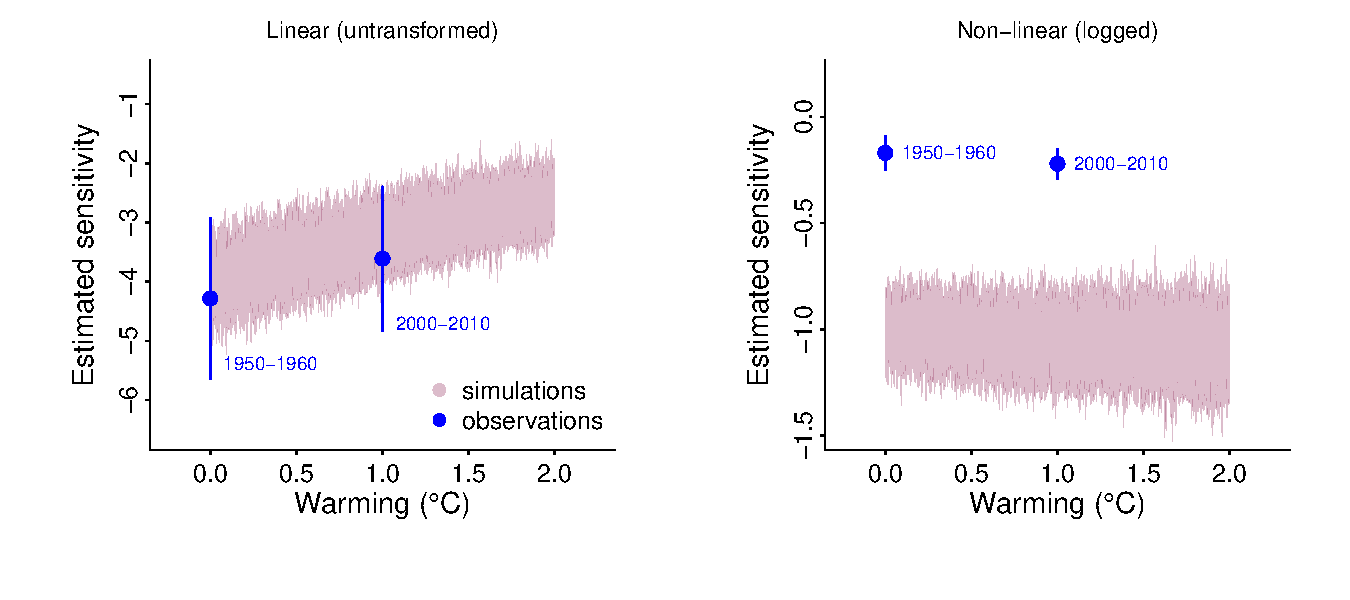
\includegraphics[width=1.05\textwidth]{..//analyses/figures/basicsimsandpepalt1.pdf} % 136 words
\caption{\textbf{Shifts in temperature sensitivities (response per $^{\circ}$C) with warming occur when using linear models for non-linear processes.} Estimated sensitivities decline (in magnitude) with warming in simulations (shading) with no underlying change in the biological process when sensitivities were estimated with linear regression (left; we simulated leafout for 45 sites as occurring after a certain thermal sum is met, simulating spring temperatures using draws from a normal(6,4), variation comes from fluctuation in the Monte Carlo simulations). This decline disappears when performing the regression on logged predictor and response variables (right). Such issues may underlie declining sensitivities calculated from observational data, including long-term observations of leafout across Europe (for \emph{Betula pendula} from PEP725 from for the 45 sites that had complete data for 1950-1960 and 2000-2010), which show a lower sensitivity with warming when calculated on raw data, but no change in sensitivity using logged data. Shading, symbols and lines represent means $\pm$ standard deviations of regressions across sites. See Supporting Information for a discussion of why estimated sensitivities are -1 in simulations in non-linear models.} % Estimates of sensitivities from logged variables were generally much lower than -1, suggesting other factors or a better metric of temperature underlie leafout dates.
\label{fig:basicsimswpep} % decsensSims.R
\end{figure}


\end{document}

